\documentclass{article}
\setlength{\parindent}{0pt}
\setlength{\parskip}{2ex plus 0.5ex minus 0.2ex}
\usepackage[margin=1in]{geometry}
\renewcommand{\topfraction}{0.9}
\renewcommand{\bottomfraction}{0.8}
\setcounter{topnumber}{2}
\setcounter{bottomnumber}{2}
\setcounter{totalnumber}{4}
\renewcommand{\textfraction}{0.07}
\renewcommand{\floatpagefraction}{0.7}
\usepackage{graphicx}
\usepackage{textcomp}
\usepackage{placeins}
\usepackage[T1]{fontenc}
\usepackage{gensymb}
\usepackage[utf8]{inputenc}
\usepackage{caption}
\usepackage[export]{adjustbox}
\graphicspath{{./figures/}}
% hyperref usually has to go last
\usepackage[hidelinks]{hyperref}
% but glossaries behaves best if after hyperref
\usepackage[acronym,toc]{glossaries}
%\newacronym{<++>}{<++>}{<++>}
\newacronym[longplural={metric tons of heavy metal}]{MTHM}{MTHM}{metric ton of heavy metal}
\newacronym{ABM}{ABM}{agent-based modeling}
\newacronym{ACDIS}{ACDIS}{Program in Arms Control \& Domestic and International Security}
\newacronym{AHTR}{AHTR}{Advanced High Temperature Reactor}
\newacronym{ANDRA}{ANDRA}{Agence Nationale pour la gestion des D\'echets RAdioactifs, the French National Agency for Radioactive Waste Management}
\newacronym{ANL}{ANL}{Argonne National Laboratory}
\newacronym{ANS}{ANS}{American Nuclear Society}
\newacronym{API}{API}{application programming interface}
\newacronym{ARE}{ARE}{Aircraft Reactor Experiment}
\newacronym{ARFC}{ARFC}{Advanced Reactors and Fuel Cycles}
\newacronym{ASME}{ASME}{American Society of Mechanical Engineers}
\newacronym{ATWS}{ATWS}{Anticipated Transient Without Scram}
\newacronym{BDBE}{BDBE}{Beyond Design Basis Event}
\newacronym{BIDS}{BIDS}{Berkeley Institute for Data Science}
\newacronym{CAFCA}{CAFCA}{ Code for Advanced Fuel Cycles Assessment }
\newacronym{CDTN}{CDTN}{Centro de Desenvolvimento da Tecnologia Nuclear}
\newacronym{CEA}{CEA}{Commissariat \`a l'\'Energie Atomique et aux \'Energies Alternatives}
\newacronym{CI}{CI}{continuous integration}
\newacronym{CNEN}{CNEN}{Comiss\~{a}o Nacional de Energia Nuclear}
\newacronym{CNERG}{CNERG}{Computational Nuclear Engineering Research Group}
\newacronym{COSI}{COSI}{Commelini-Sicard}
\newacronym{COTS}{COTS}{commercial, off-the-shelf}
\newacronym{CSNF}{CSNF}{commercial spent nuclear fuel}
\newacronym{CTAH}{CTAHs}{Coiled Tube Air Heaters}
\newacronym{CUBIT}{CUBIT}{CUBIT Geometry and Mesh Generation Toolkit}
\newacronym{CURIE}{CURIE}{Centralized Used Fuel Resource for Information Exchange}
\newacronym{DAG}{DAG}{directed acyclic graph}
\newacronym{DANESS}{DANESS}{Dynamic Analysis of Nuclear Energy System Strategies}
\newacronym{DBE}{DBE}{Design Basis Event}
\newacronym{DESAE}{DESAE}{Dynamic Analysis of Nuclear Energy Systems Strategies}
\newacronym{DHS}{DHS}{Department of Homeland Security}
\newacronym{DOE}{DOE}{Department of Energy}
\newacronym{DRACS}{DRACS}{Direct Reactor Auxiliary Cooling System}
\newacronym{DRE}{DRE}{dynamic resource exchange}
\newacronym{DSNF}{DSNF}{DOE spent nuclear fuel}
\newacronym{DYMOND}{DYMOND}{Dynamic Model of Nuclear Development }
\newacronym{EBS}{EBS}{Engineered Barrier System}
\newacronym{EDF}{EDF}{Électricité de France}
\newacronym{EDZ}{EDZ}{Excavation Disturbed Zone}
\newacronym{EIA}{EIA}{U.S. Energy Information Administration}
\newacronym{EPA}{EPA}{Environmental Protection Agency}
\newacronym{EPR}{EPR}{European Pressurized Reactors}
\newacronym{EP}{EP}{Engineering Physics}
\newacronym{EU}{EU}{European Union}
\newacronym{FCO}{FCO}{Fuel Cycle Options}
\newacronym{FCT}{FCT}{Fuel Cycle Technology}
\newacronym{FEHM}{FEHM}{Finite Element Heat and Mass Transfer}
\newacronym{FEPs}{FEPs}{Features, Events, and Processes}
\newacronym{FHR}{FHR}{Fluoride-Salt-Cooled High-Temperature Reactor}
\newacronym{FLiBe}{FLiBe}{Fluoride-Lithium-Beryllium}
\newacronym{FP}{FP}{Fission Products}
\newacronym{GDSE}{GDSE}{Generic Disposal System Environment}
\newacronym{GDSM}{GDSM}{Generic Disposal System Model}
\newacronym{GENIUSv1}{GENIUSv1}{Global Evaluation of Nuclear Infrastructure Utilization Scenarios, Version 1}
\newacronym{GENIUSv2}{GENIUSv2}{Global Evaluation of Nuclear Infrastructure Utilization Scenarios, Version 2}
\newacronym{GENIUS}{GENIUS}{Global Evaluation of Nuclear Infrastructure Utilization Scenarios}
\newacronym{GPAM}{GPAM}{Generic Performance Assessment Model}
\newacronym{GRSAC}{GRSAC}{Graphite Reactor Severe Accident Code}
\newacronym{GUI}{GUI}{graphical user interface}
\newacronym{HLW}{HLW}{high level waste}
\newacronym{HPC}{HPC}{high-performance computing}
\newacronym{HTC}{HTC}{high-throughput computing}
\newacronym{HTGR}{HTGR}{High Temperature Gas-Cooled Reactor}
\newacronym{IAEA}{IAEA}{International Atomic Energy Agency}
\newacronym{IEMA}{IEMA}{Illinois Emergency Mangament Agency}
\newacronym{IHLRWM}{IHLRWM}{International High Level Radioactive Waste Management}
\newacronym{INL}{INL}{Idaho National Laboratory}
\newacronym{IPRR1}{IRP-R1}{Instituto de Pesquisas Radioativas Reator 1}
\newacronym{IRP}{IRP}{Integrated Research Project}
\newacronym{ISFSI}{ISFSI}{Independent Spent Fuel Storage Installation}
\newacronym{ISRG}{ISRG}{Independent Student Research Group}
\newacronym{JFNK}{JFNK}{Jacobian-Free Newton Krylov}
\newacronym{LANL}{LANL}{Los Alamos National Laboratory}
\newacronym{LBNL}{LBNL}{Lawrence Berkeley National Laboratory}
\newacronym{LCOE}{LCOE}{levelized cost of electricity}
\newacronym{LDRD}{LDRD}{laboratory directed research and development}
\newacronym{LFR}{LFR}{Lead-Cooled Fast Reactor}
\newacronym{LLNL}{LLNL}{Lawrence Livermore National Laboratory}
\newacronym{LMFBR}{LMFBR}{Liquid Metal Fast Breeder Reactor}
\newacronym{LOFC}{LOFC}{Loss of Forced Cooling}
\newacronym{LOHS}{LOHS}{Loss of Heat Sink}
\newacronym{LOLA}{LOLA}{Loss of Large Area}
\newacronym{LP}{LP}{linear program}
\newacronym{LWR}{LWR}{Light Water Reactor}
\newacronym{MAGNOX}{MAGNOX}{Magnesium Alloy Graphie Moderated Gas Cooled Uranium Oxide Reactor}
\newacronym{MA}{MA}{minor actinide}
\newacronym{MCNP}{MCNP}{Monte Carlo N-Particle code}
\newacronym{MILP}{MILP}{mixed-integer linear program}
\newacronym{MIT}{MIT}{the Massachusetts Institute of Technology}
\newacronym{MOAB}{MOAB}{Mesh-Oriented datABase}
\newacronym{MOOSE}{MOOSE}{Multiphysics Object-Oriented Simulation Environment}
\newacronym{MOX}{MOX}{mixed oxide}
\newacronym{MSBR}{MSBR}{Molten Salt Breeder Reactor}
\newacronym{MSRE}{MSRE}{Molten Salt Reactor Experiment}
\newacronym{MSR}{MSR}{Molten Salt Reactor}
\newacronym{NAGRA}{NAGRA}{National Cooperative for the Disposal of Radioactive Waste}
\newacronym{NEAMS}{NEAMS}{Nuclear Engineering Advanced Modeling and Simulation}
\newacronym{NEUP}{NEUP}{Nuclear Energy University Programs}
\newacronym{NFCSim}{NFCSim}{Nuclear Fuel Cycle Simulator}
\newacronym{NGNP}{NGNP}{Next Generation Nuclear Plant}
\newacronym{NMWPC}{NMWPC}{Nuclear MW Per Capita}
\newacronym{NNSA}{NNSA}{National Nuclear Security Administration}
\newacronym{NPP}{NPP}{Nuclear Power Plant}
\newacronym{NPRE}{NPRE}{Department of Nuclear, Plasma, and Radiological Engineering}
\newacronym{NQA1}{NQA-1}{Nuclear Quality Assurance - 1}
\newacronym{NRC}{NRC}{Nuclear Regulatory Commission}
\newacronym{NSF}{NSF}{National Science Foundation}
\newacronym{NSSC}{NSSC}{Nuclear Science and Security Consortium}
\newacronym{NUWASTE}{NUWASTE}{Nuclear Waste Assessment System for Technical Evaluation}
\newacronym{NWF}{NWF}{Nuclear Waste Fund}
\newacronym{NWTRB}{NWTRB}{Nuclear Waste Technical Review Board}
\newacronym{OCRWM}{OCRWM}{Office of Civilian Radioactive Waste Management}
\newacronym{ORION}{ORION}{ORION}
\newacronym{ORNL}{ORNL}{Oak Ridge National Laboratory}
\newacronym{PARCS}{PARCS}{Purdue Advanced Reactor Core Simulator}
\newacronym{PBAHTR}{PB-AHTR}{Pebble Bed Advanced High Temperature Reactor}
\newacronym{PBFHR}{PB-FHR}{Pebble-Bed Fluoride-Salt-Cooled High-Temperature Reactor}
\newacronym{PEI}{PEI}{Peak Environmental Impact}
\newacronym{PH}{PRONGHORN}{PRONGHORN}
\newacronym{PRIS}{PRIS}{Power Reactor Information System}
\newacronym{PRKE}{PRKE}{Point Reactor Kinetics Equations}
\newacronym{PSPG}{PSPG}{Pressure-Stabilizing/Petrov-Galerkin}
\newacronym{PWAR}{PWAR}{Pratt and Whitney Aircraft Reactor}
\newacronym{PWR}{PWR}{Pressurized Water Reactor}
\newacronym{PyNE}{PyNE}{Python toolkit for Nuclear Engineering}
\newacronym{PyRK}{PyRK}{Python for Reactor Kinetics}
\newacronym{QA}{QA}{quality assurance}
\newacronym{RDD}{RD\&D}{Research Development and Demonstration}
\newacronym{RD}{R\&D}{Research and Development}
\newacronym{RELAP}{RELAP}{Reactor Excursion and Leak Analysis Program}
\newacronym{RIA}{RIA}{Reactivity Insertion Accident}
\newacronym{RIF}{RIF}{Region-Institution-Facility}
\newacronym{SFR}{SFR}{Sodium-Cooled Fast Reactor}
\newacronym{SINDAG}{SINDA{\textbackslash}G}{Systems Improved Numerical Differencing Analyzer $\backslash$ Gaski}
\newacronym{SKB}{SKB}{Svensk K\"{a}rnbr\"{a}nslehantering AB}
\newacronym{SNF}{SNF}{spent nuclear fuel}
\newacronym{SNL}{SNL}{Sandia National Laboratory}
\newacronym{STC}{STC}{specific temperature change}
\newacronym{SUPG}{SUPG}{Streamline-Upwind/Petrov-Galerkin}
\newacronym{SWF}{SWF}{Separations and Waste Forms}
\newacronym{SWU}{SWU}{Separative Work Unit}
\newacronym{TRIGA}{TRIGA}{Training Research Isotope General Atomic}
\newacronym{TRISO}{TRISO}{Tristructural Isotropic}
\newacronym{TSM}{TSM}{Total System Model}
\newacronym{TSPA}{TSPA}{Total System Performance Assessment for the Yucca Mountain License Application}
\newacronym{ThOX}{ThOX}{thorium oxide}
\newacronym{UFD}{UFD}{Used Fuel Disposition}
\newacronym{UML}{UML}{Unified Modeling Language}
\newacronym{UOX}{UOX}{uranium oxide}
\newacronym{UQ}{UQ}{uncertainty quantification}
\newacronym{US}{US}{United States}
\newacronym{UW}{UW}{University of Wisconsin}
\newacronym{VISION}{VISION}{the Verifiable Fuel Cycle Simulation Model}
\newacronym{VVER}{VVER}{Voda-Vodyanoi Energetichesky Reaktor (Russian Pressurized Water Reactor)}
\newacronym{VV}{V\&V}{verification and validation}
\newacronym{WIPP}{WIPP}{Waste Isolation Pilot Plant}
\newacronym{YMR}{YMR}{Yucca Mountain Repository Site}

\makeglossaries
% cleveref only behaves if after hyperref & glossaries
\usepackage{cleveref}

\let\Oldsection\section
\renewcommand{\section}{\FloatBarrier\Oldsection}

\let\Oldsubsection\subsection
\renewcommand{\subsection}{\FloatBarrier\Oldsubsection}

\let\Oldsubsubsection\subsubsection
\renewcommand{\subsubsection}{\FloatBarrier\Oldsubsubsection}

\newcommand{\code}[1]{\texttt{#1}}

\title{Introduction to Moltres: an Application for Simulation of Molten Salt Reactors}
\author{Alexander Lindsay, Kathryn Huff}

\begin{document}
\maketitle

\section{Model Description}

Neutrons are described with time-dependent multi-group diffusion theory as shown
in \cref{eq:neutrons}:

\begin{equation}
%% \frac{1}{v_g}\frac{\partial \phi_g}{\partial t} - \nabla \cdot D_g \nabla \phi_g
%% + \Sigma_g^r \phi_g = \sum_{g \ne g'}^G \Sigma_{g'\rightarrow g}^s \phi_{g'} + \chi_g^p \sum_{g' = 1}^G (1 - \beta)
%% \nu \Sigma_{g'}^f \phi_{g'}
\frac{1}{v_g}\frac{\partial \phi_g}{\partial t} - \nabla \cdot D_g \nabla \phi_g
+ \Sigma_g^r \phi_g = \sum_{g \ne g'}^G \Sigma_{g'\rightarrow g}^s \phi_{g'} + \chi_g^p \sum_{g' = 1}^G (1 - \beta)
\nu \Sigma_{g'}^f \phi_{g'} + \chi_g^d \sum_i^I \lambda_i C_i
\label{eq:neutrons}
\end{equation}

Delayed neutron precursors are described by \cref{eq:precursors}:

\begin{equation}
\frac{\partial C_i}{\partial t} = \sum_{g'= 1}^G \beta_i \nu \Sigma_{g'}^f
\phi_{g'} - \lambda_i C_i - \frac{\partial}{\partial z} u C_i
\label{eq:precursors}
\end{equation}

with the last term representing the effect of fuel advection. The governing
equation for the temperature is given by:

\begin{equation}
  \rho_fc_{p,f}\frac{\partial T_f}{\partial t} + \nabla\cdot\left(\rho_f c_{p,f}
  \vec{u}\cdot T_f -k_f\nabla T_f\right) =  Q_f
  \label{eq:fuel_temp}
\end{equation}

in the fuel and by:

\begin{equation}
  \rho_gc_{p,g}\frac{\partial T_g}{\partial t} + \nabla\cdot\left(-k_g\nabla T_g\right) =  Q_g
  \label{eq:moderator_temp}
\end{equation}

in the moderator. $Q_f$ is defined by:

\begin{equation}
  Q_f = \sum_{g=1}^G \epsilon_{f,g}\Sigma_{f,g}\phi_g
  \label{eq:fuel_source}
\end{equation}

and $Q_g$ is equal to $\gamma Q_f$, representing heat dissipation by gamma and
neutron irradiation in the moderator.

\section{Results \& Discussion}

\subsection{Continuous Galerkin for Temperature with Isotropic Stabilization}

\Cref{fig:cg_group1,fig:cg_group2} show expected cosinusoidal shapes for the
fast and thermal group fluxes with respect to the axial coordinate. Fast group neutrons
show a slight preference for the fuel region, while the thermal group slightly
prefers the moderator as we would intuitively expect.

%% \begin{figure}[H]
\begin{figure}[htpb]
  \centering
  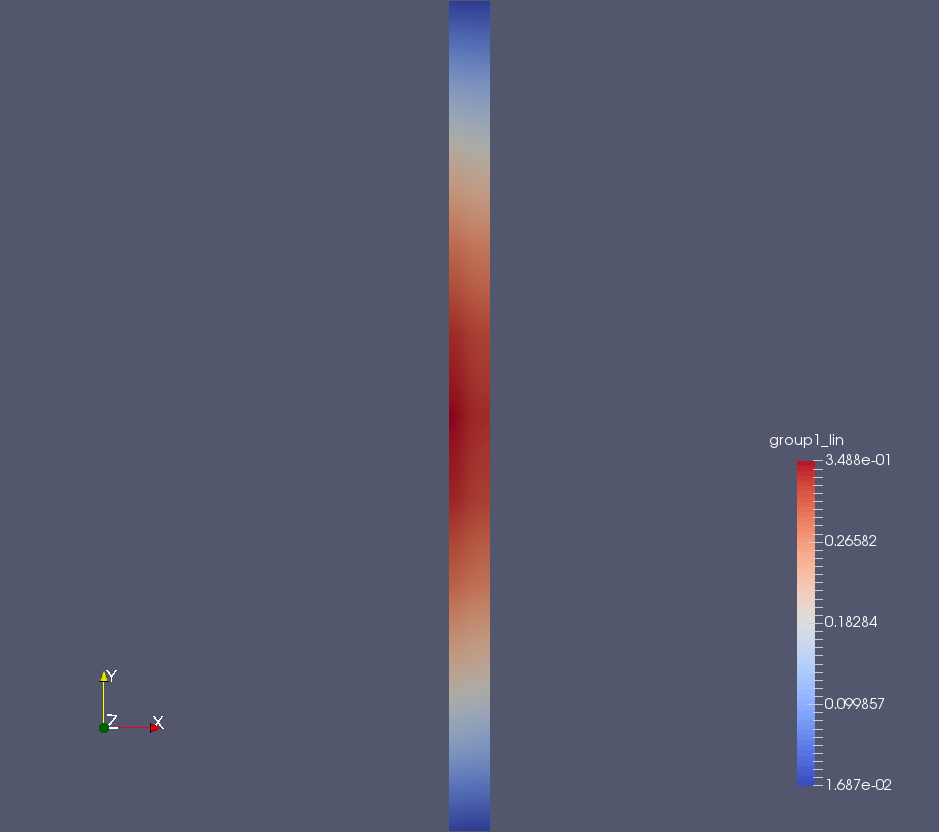
\includegraphics[width=.5\textwidth]{nt_group_1.png}
  \caption{Fast group neutron flux for Continuous Galerkin discretization}
  \label{fig:cg_group1}
\end{figure}

%% \begin{figure}[H]
\begin{figure}[htpb]
  \centering
  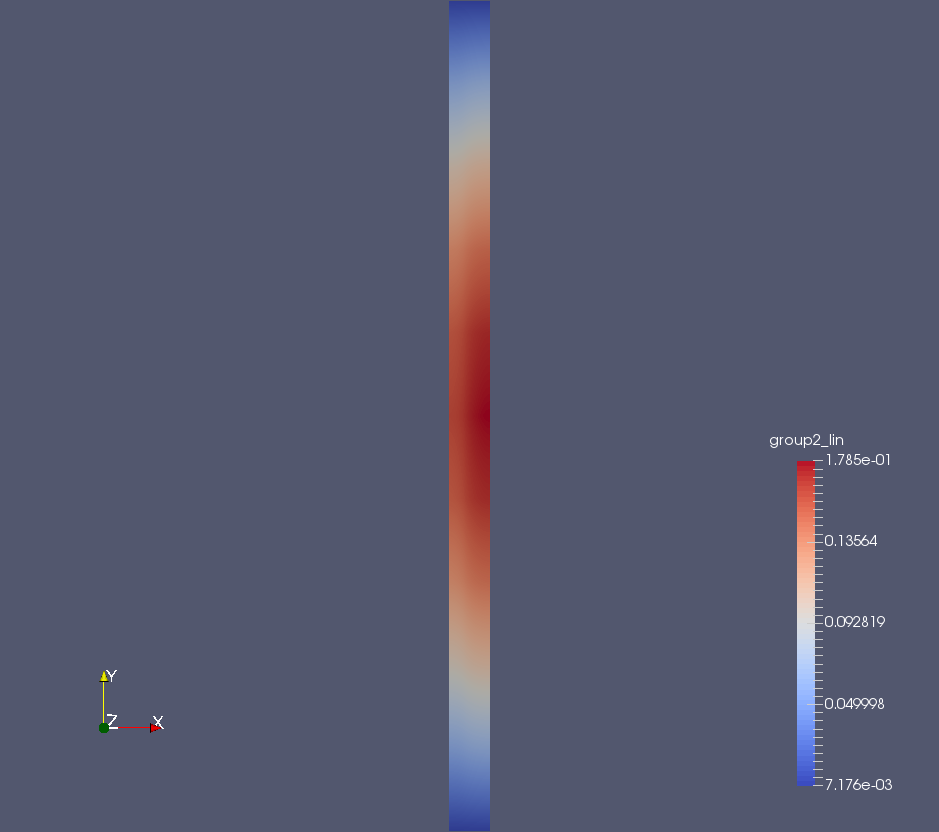
\includegraphics[width=.5\textwidth]{nt_group_2.png}
  \caption{Thermal group neutron flux for Continuous Galerkin discretization}
  \label{fig:cg_group2}
\end{figure}

In \cref{fig:cg_temperature} we see that the reactor outlet temperature is
around 992 K, which is within the realm of physical possiblity. The temperature
monotonically increases with increasing axial coordinate in the direction of
flow; radial profiles are uniform.

%% \begin{figure}[H]
\begin{figure}[htpb]
  \centering
  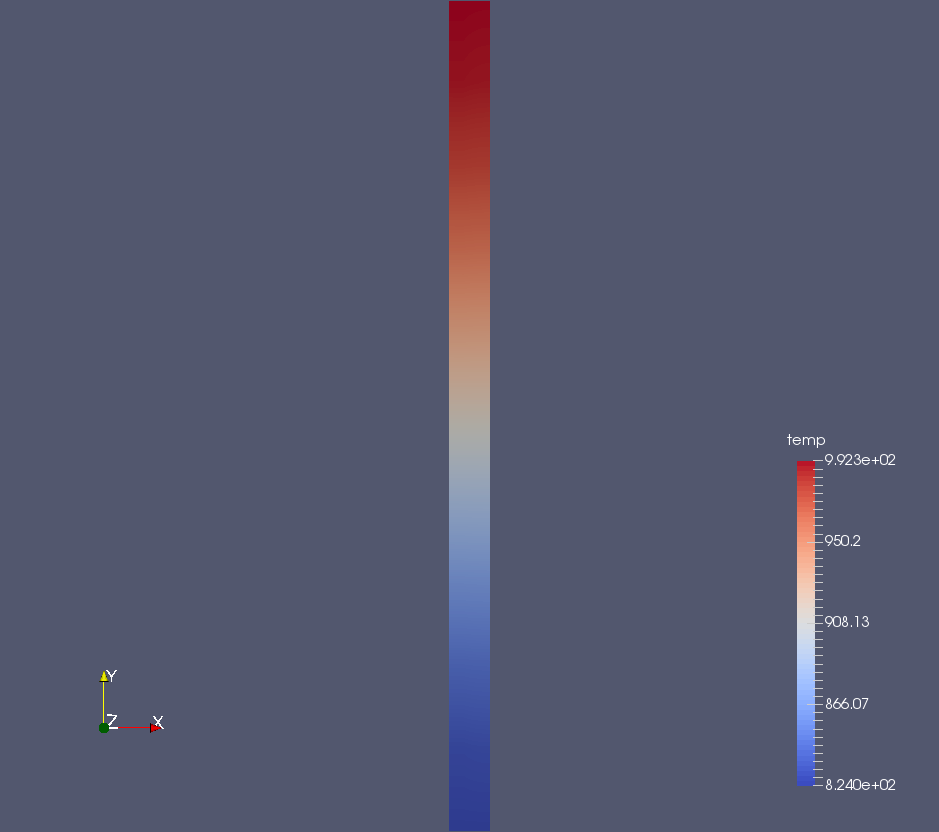
\includegraphics[width=.5\textwidth]{temperature.png}
  \caption{Temperature for Continuous Galerkin discretization}
  \label{fig:cg_temperature}
\end{figure}

\Cref{fig:cg_longest_precursor,fig:cg_shortest_precursor} show the profiles of
the longest and shortest lived precursors respectively. The longest lived
precursor concentration peaks at the reactor outlet, while the shortest lived
precursor shows a maximum concentration at approximately z = 85 cm. The use of
constant monomial basis functions for the precursor solution approximation is
evident in the elemental visualizations.

%% \begin{figure}[H]
\begin{figure}[htpb]
  \centering
  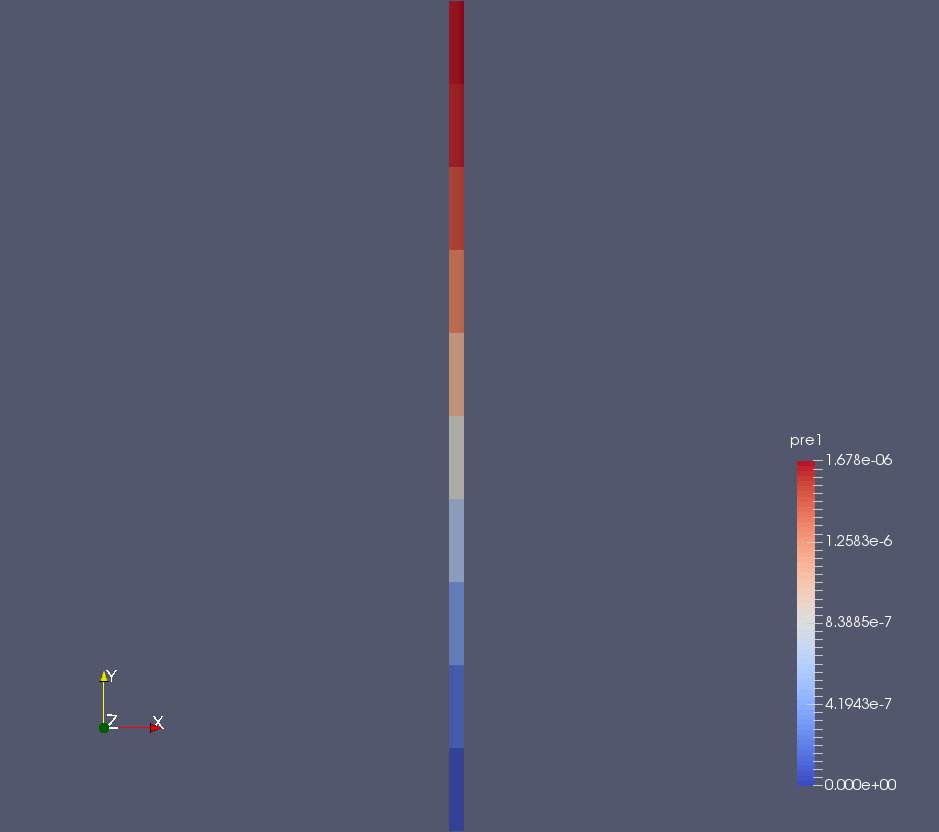
\includegraphics[width=.5\textwidth]{longest_lived_precursor.png}
  \caption{Longest lived precursor for Continuous Galerkin discretization}
  \label{fig:cg_longest_precursor}
\end{figure}

%% \begin{figure}[H]
\begin{figure}[htpb]
  \centering
  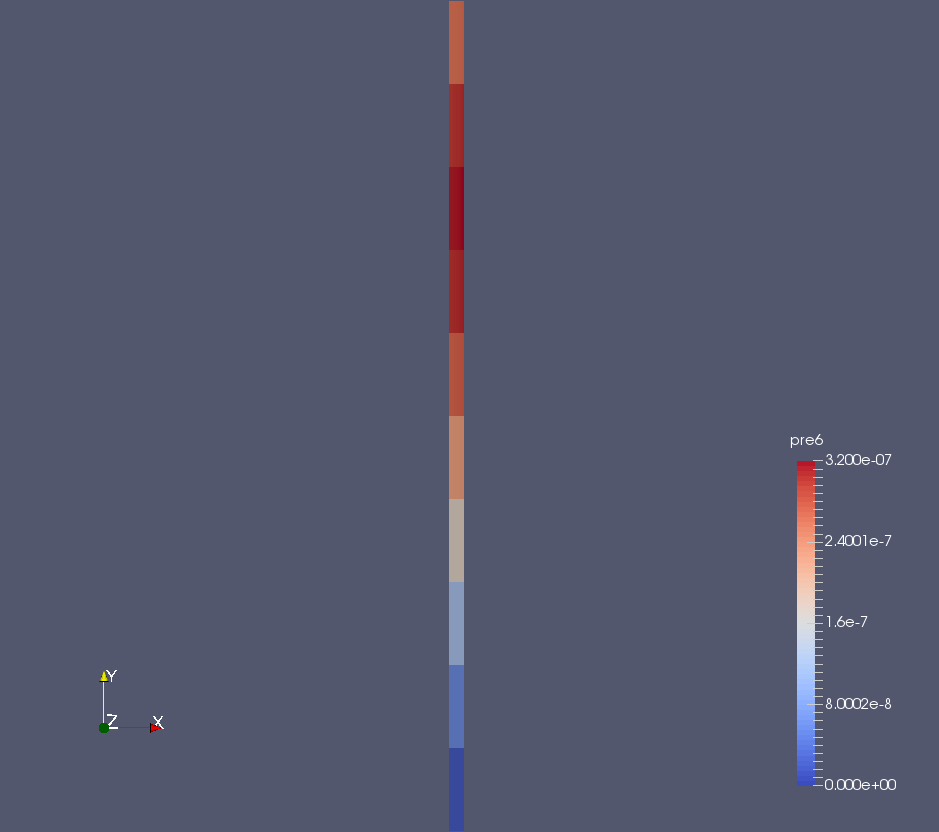
\includegraphics[width=.5\textwidth]{shortest_lived_precursor.png}
  \caption{Shortest lived precursor for Continuous Galerkin discretization}
  \label{fig:cg_shortest_precursor}
\end{figure}

\FloatBarrier

\subsection{Discontinuous Galerkin for Temperature}

Moving to a discontinuous Galerkin discretization and removing isotropic
stabilization yields a dramatically different temperature profile, as shown in
\cref{fig:dg_temperature}. With dramatically reduced heat flux due to removal of
artificial conduction, the outlet temperature of the reactor is now 1119 K,
about 130 K higher than the \gls{CG} case shown in \cref{fig:cg_temperature}.

%% \begin{figure}[H]
\begin{figure}[htpb]
  \centering
  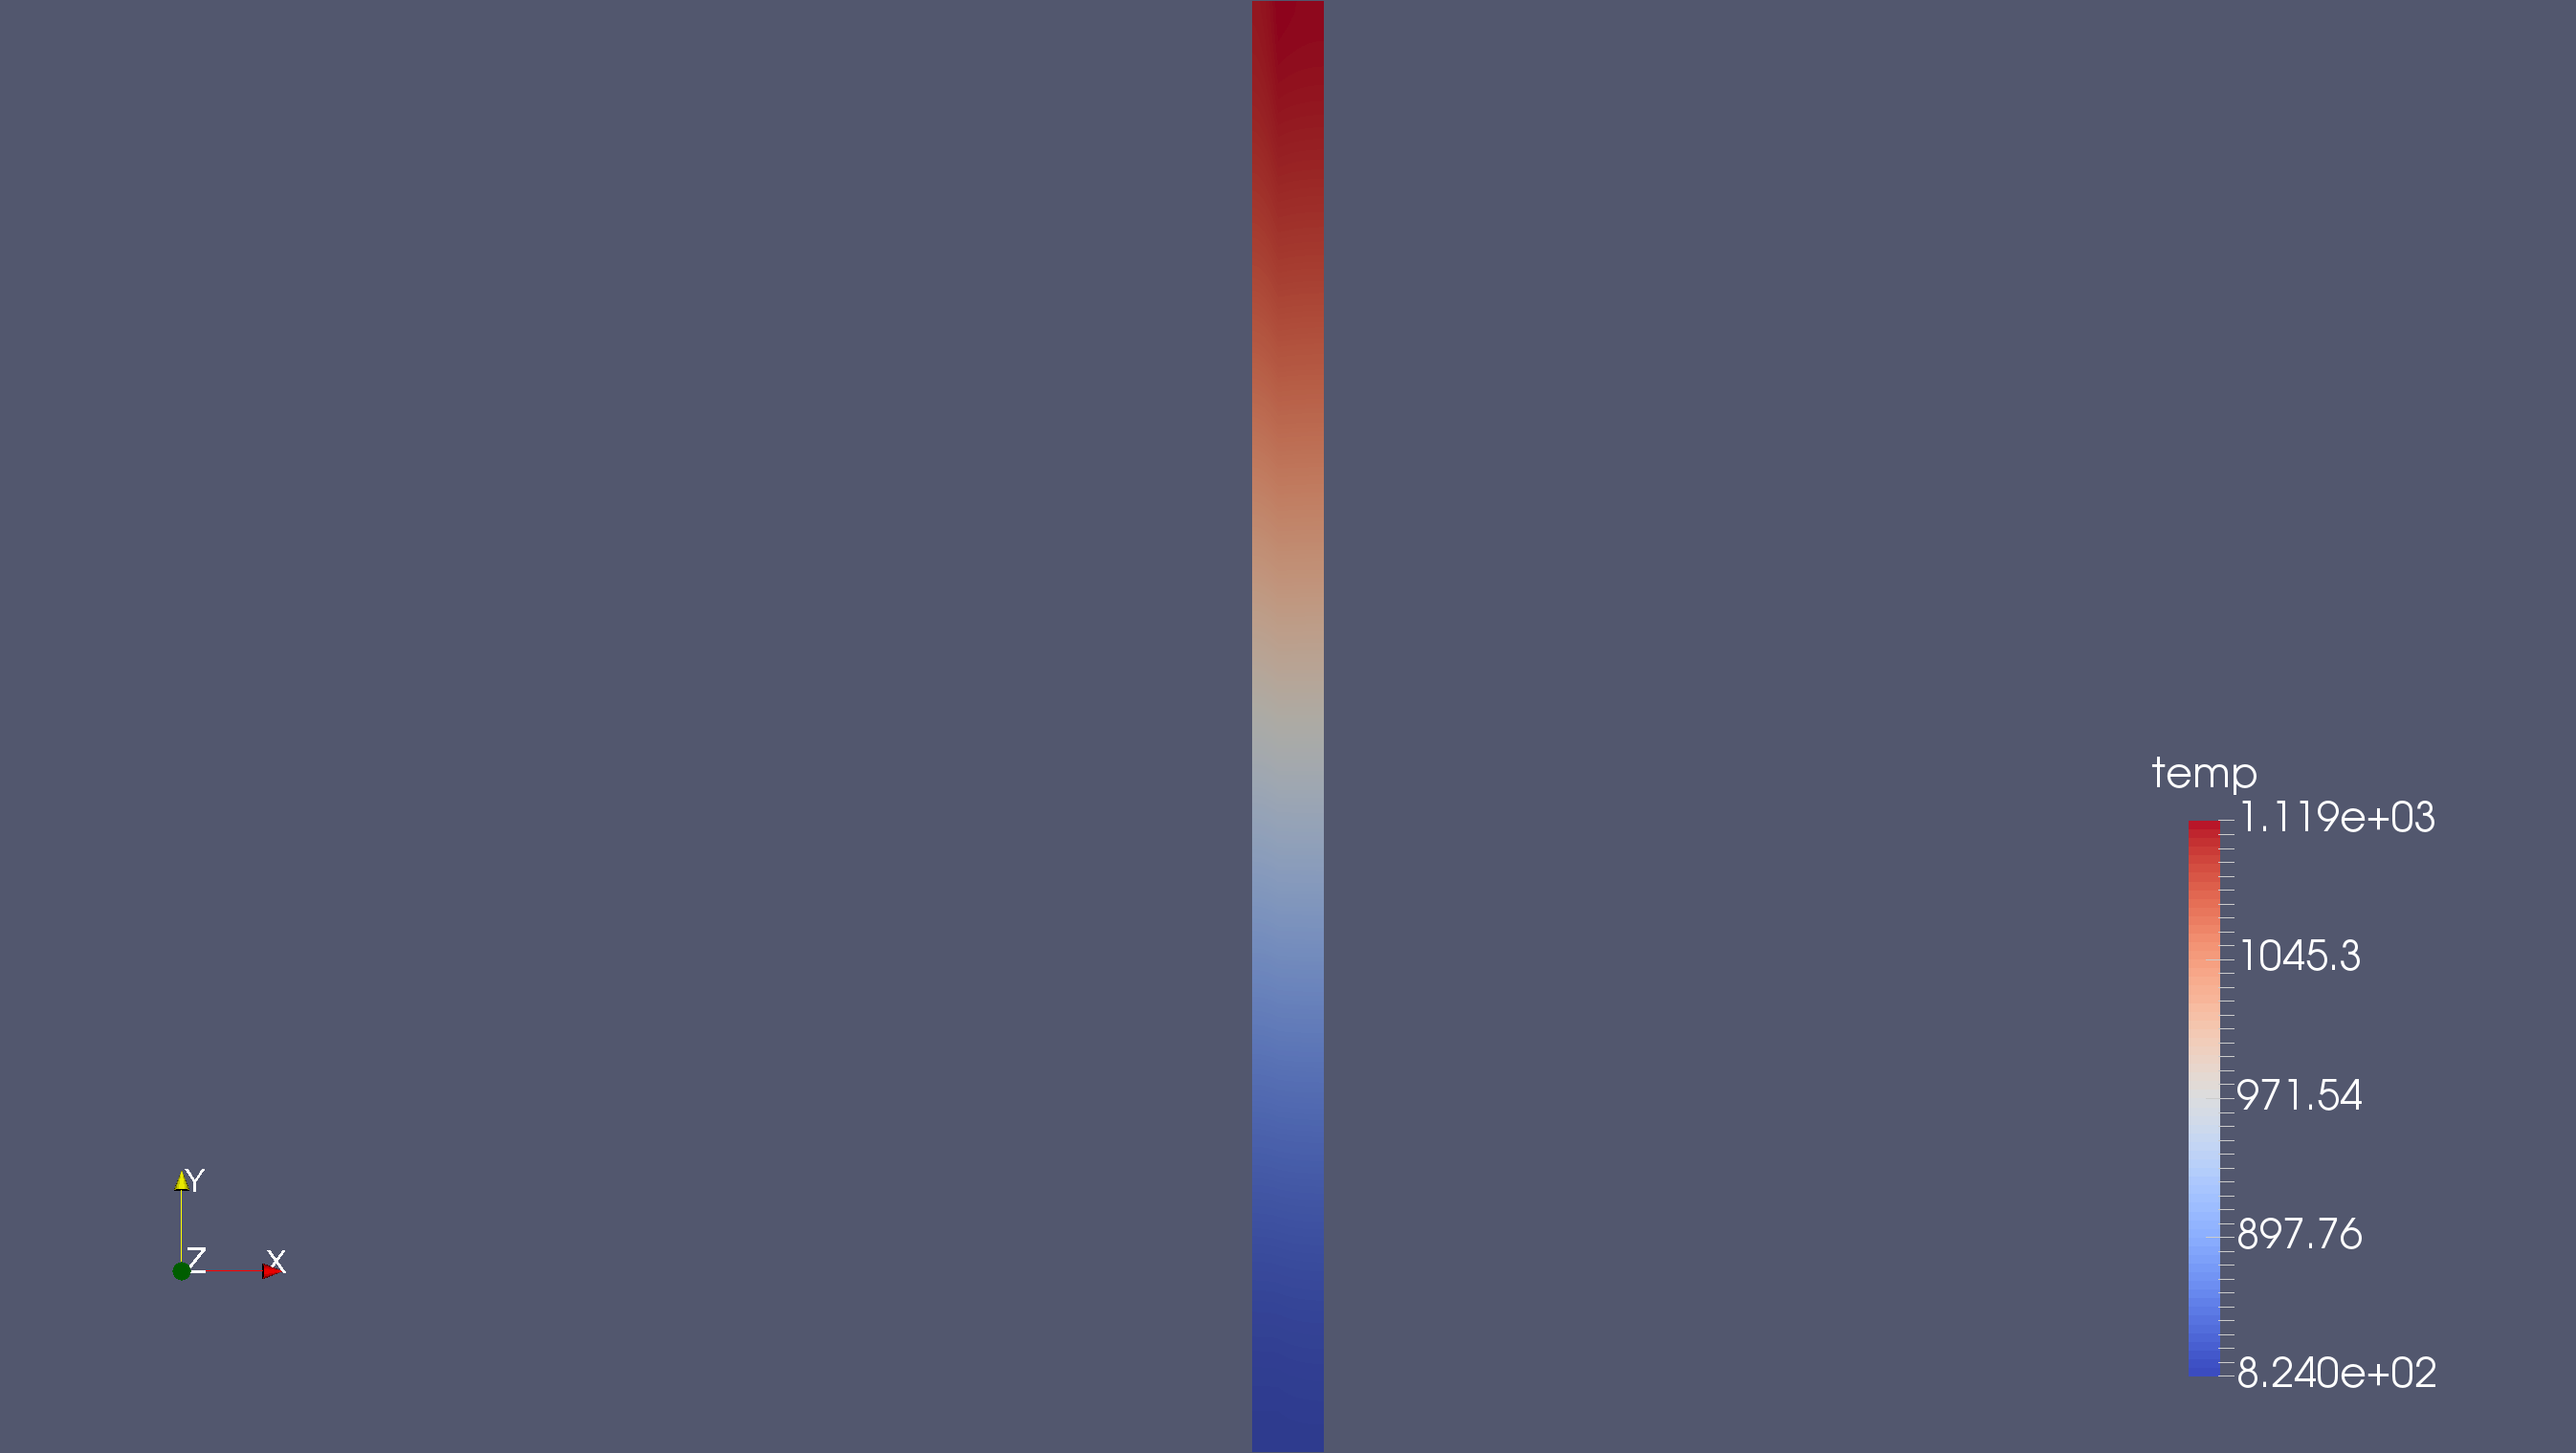
\includegraphics[width=.5\textwidth]{dg_temperature.png}
  \caption{Temperature for Discontinuous Galerkin discretization}
  \label{fig:dg_temperature}
\end{figure}

As shown in \cref{fig:dg_group1,fig:dg_group2}, the shapes of the neutron flux
distributions do not change with the move to \gls{DG}. The magnitudes of the
fluxes do increase by about 35\%.

%% \begin{figure}[H]
\begin{figure}[htpb]
  \centering
  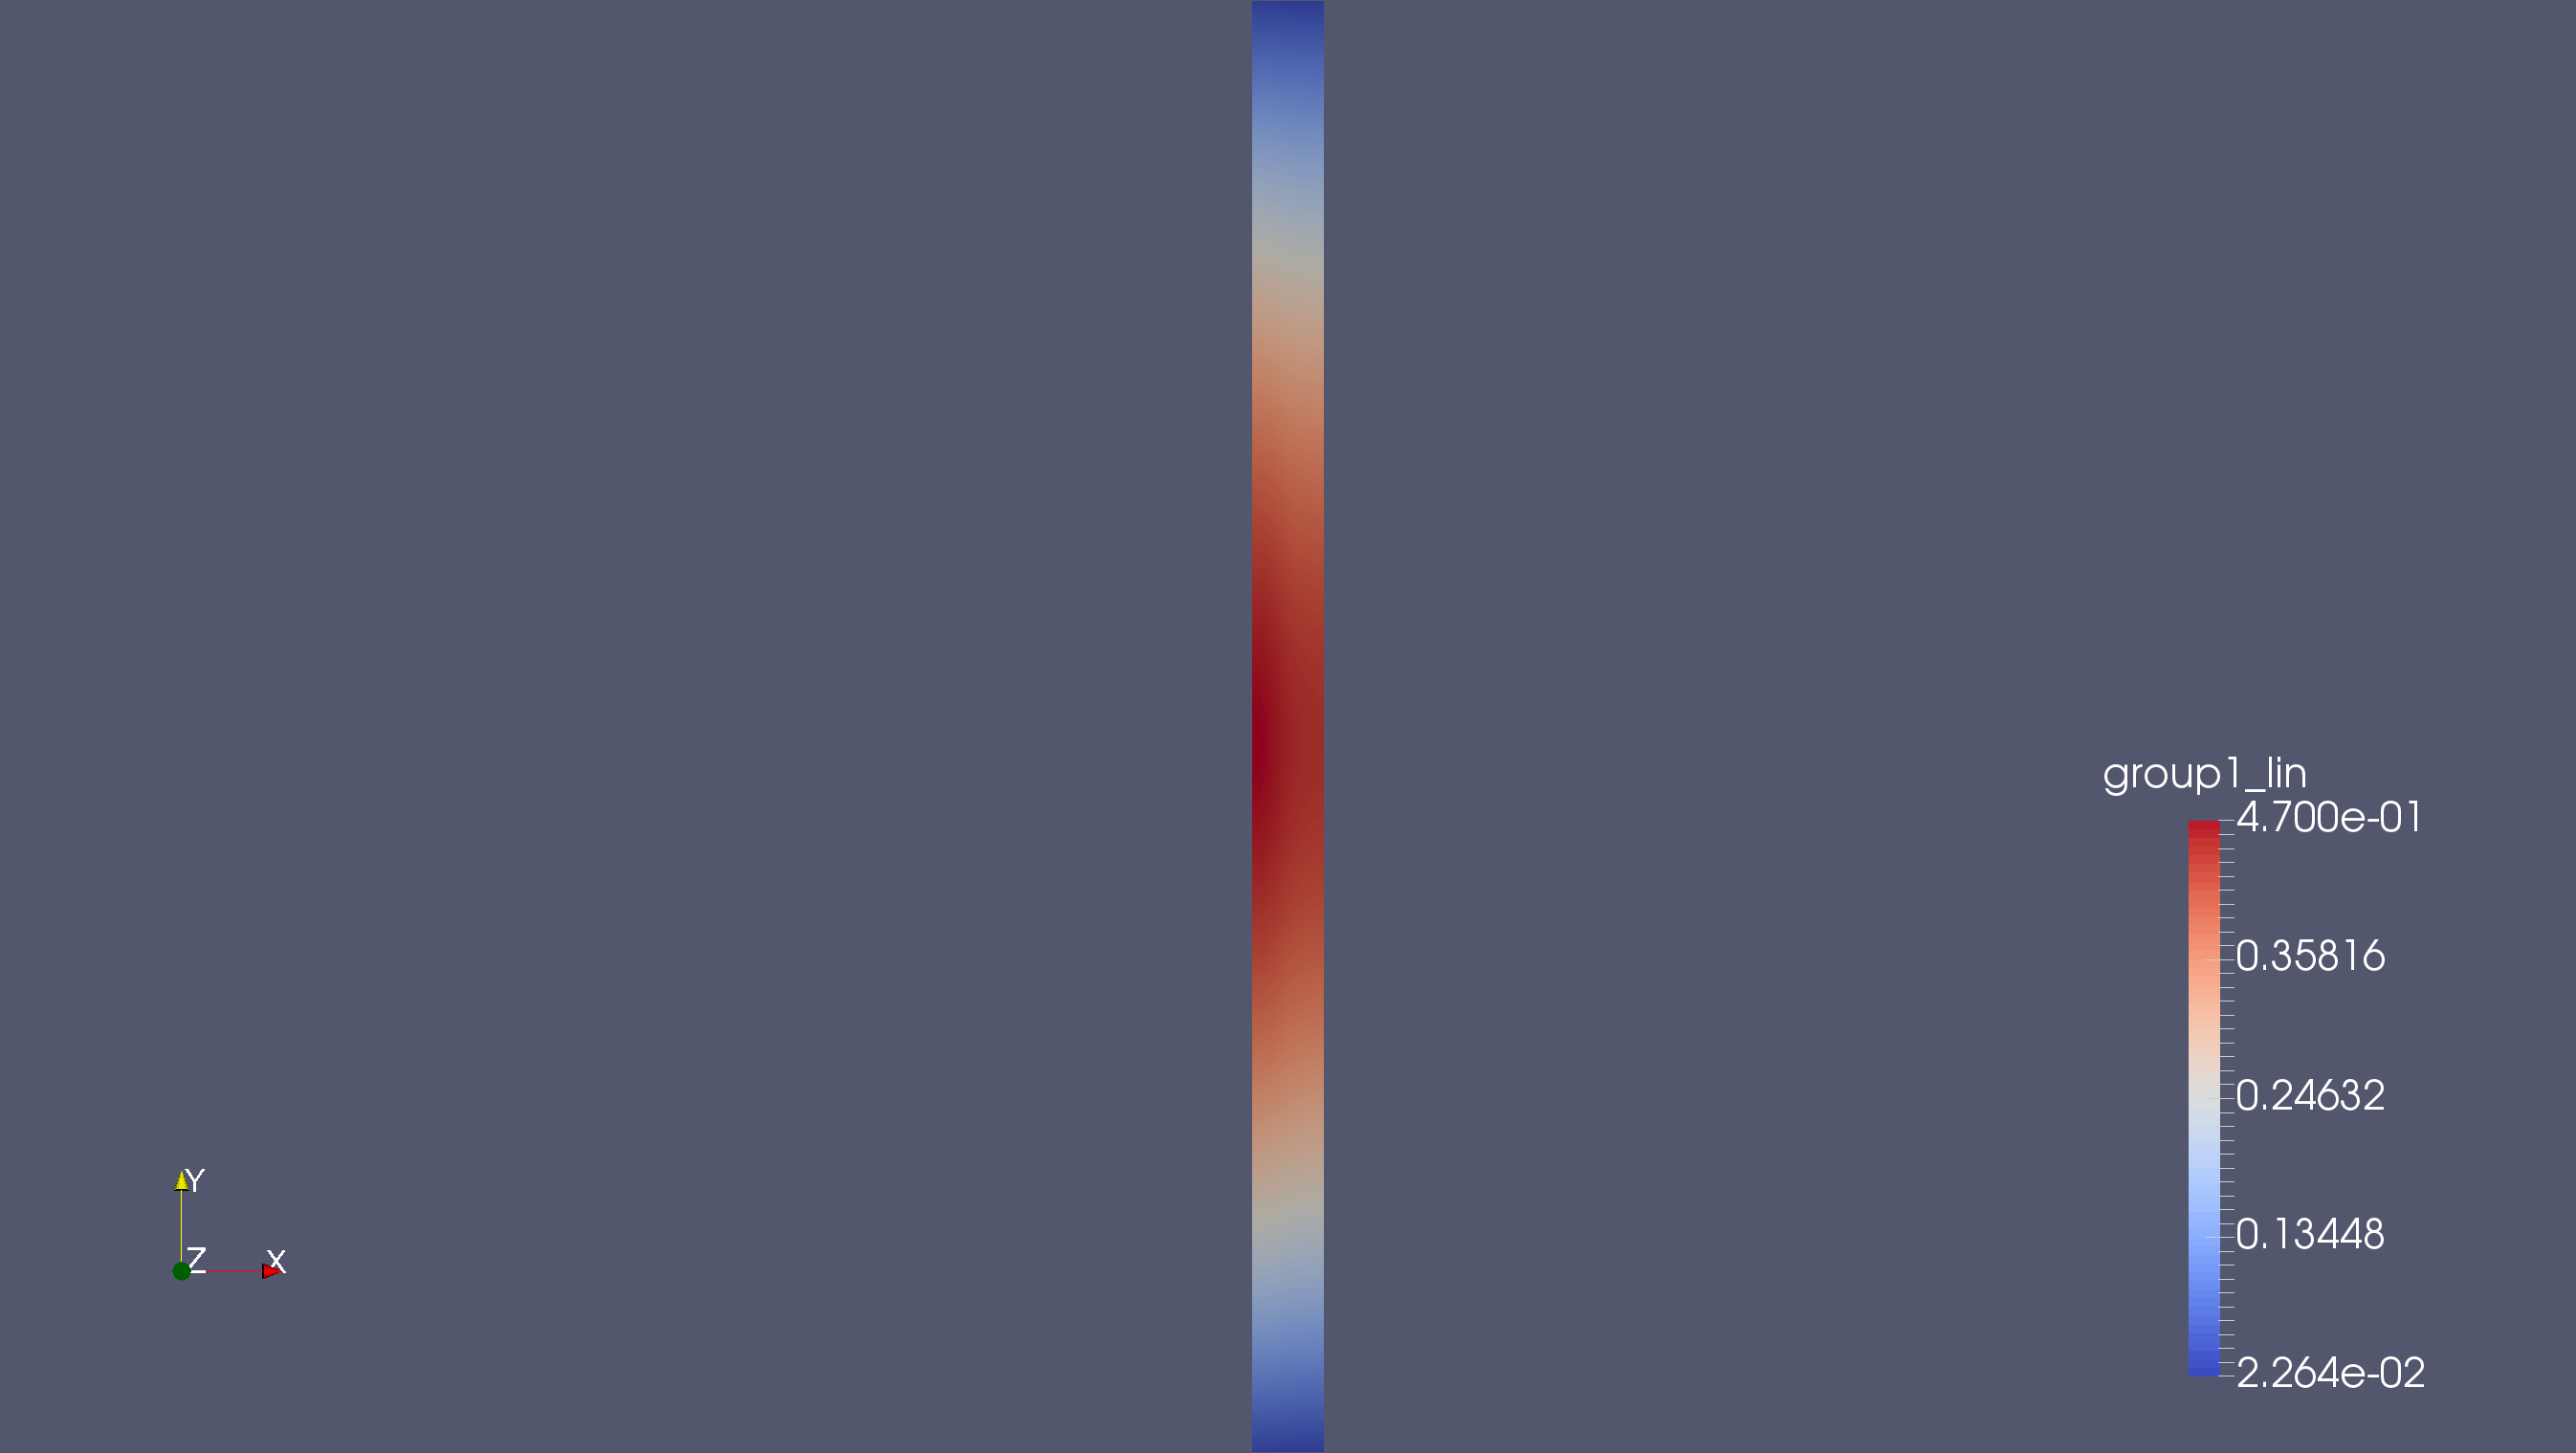
\includegraphics[width=.5\textwidth]{dg_group1.png}
  \caption{Fast group neutron flux for Discontinuous Galerkin discretization}
  \label{fig:dg_group1}
\end{figure}

%% \begin{figure}[H]
\begin{figure}[htpb]
  \centering
  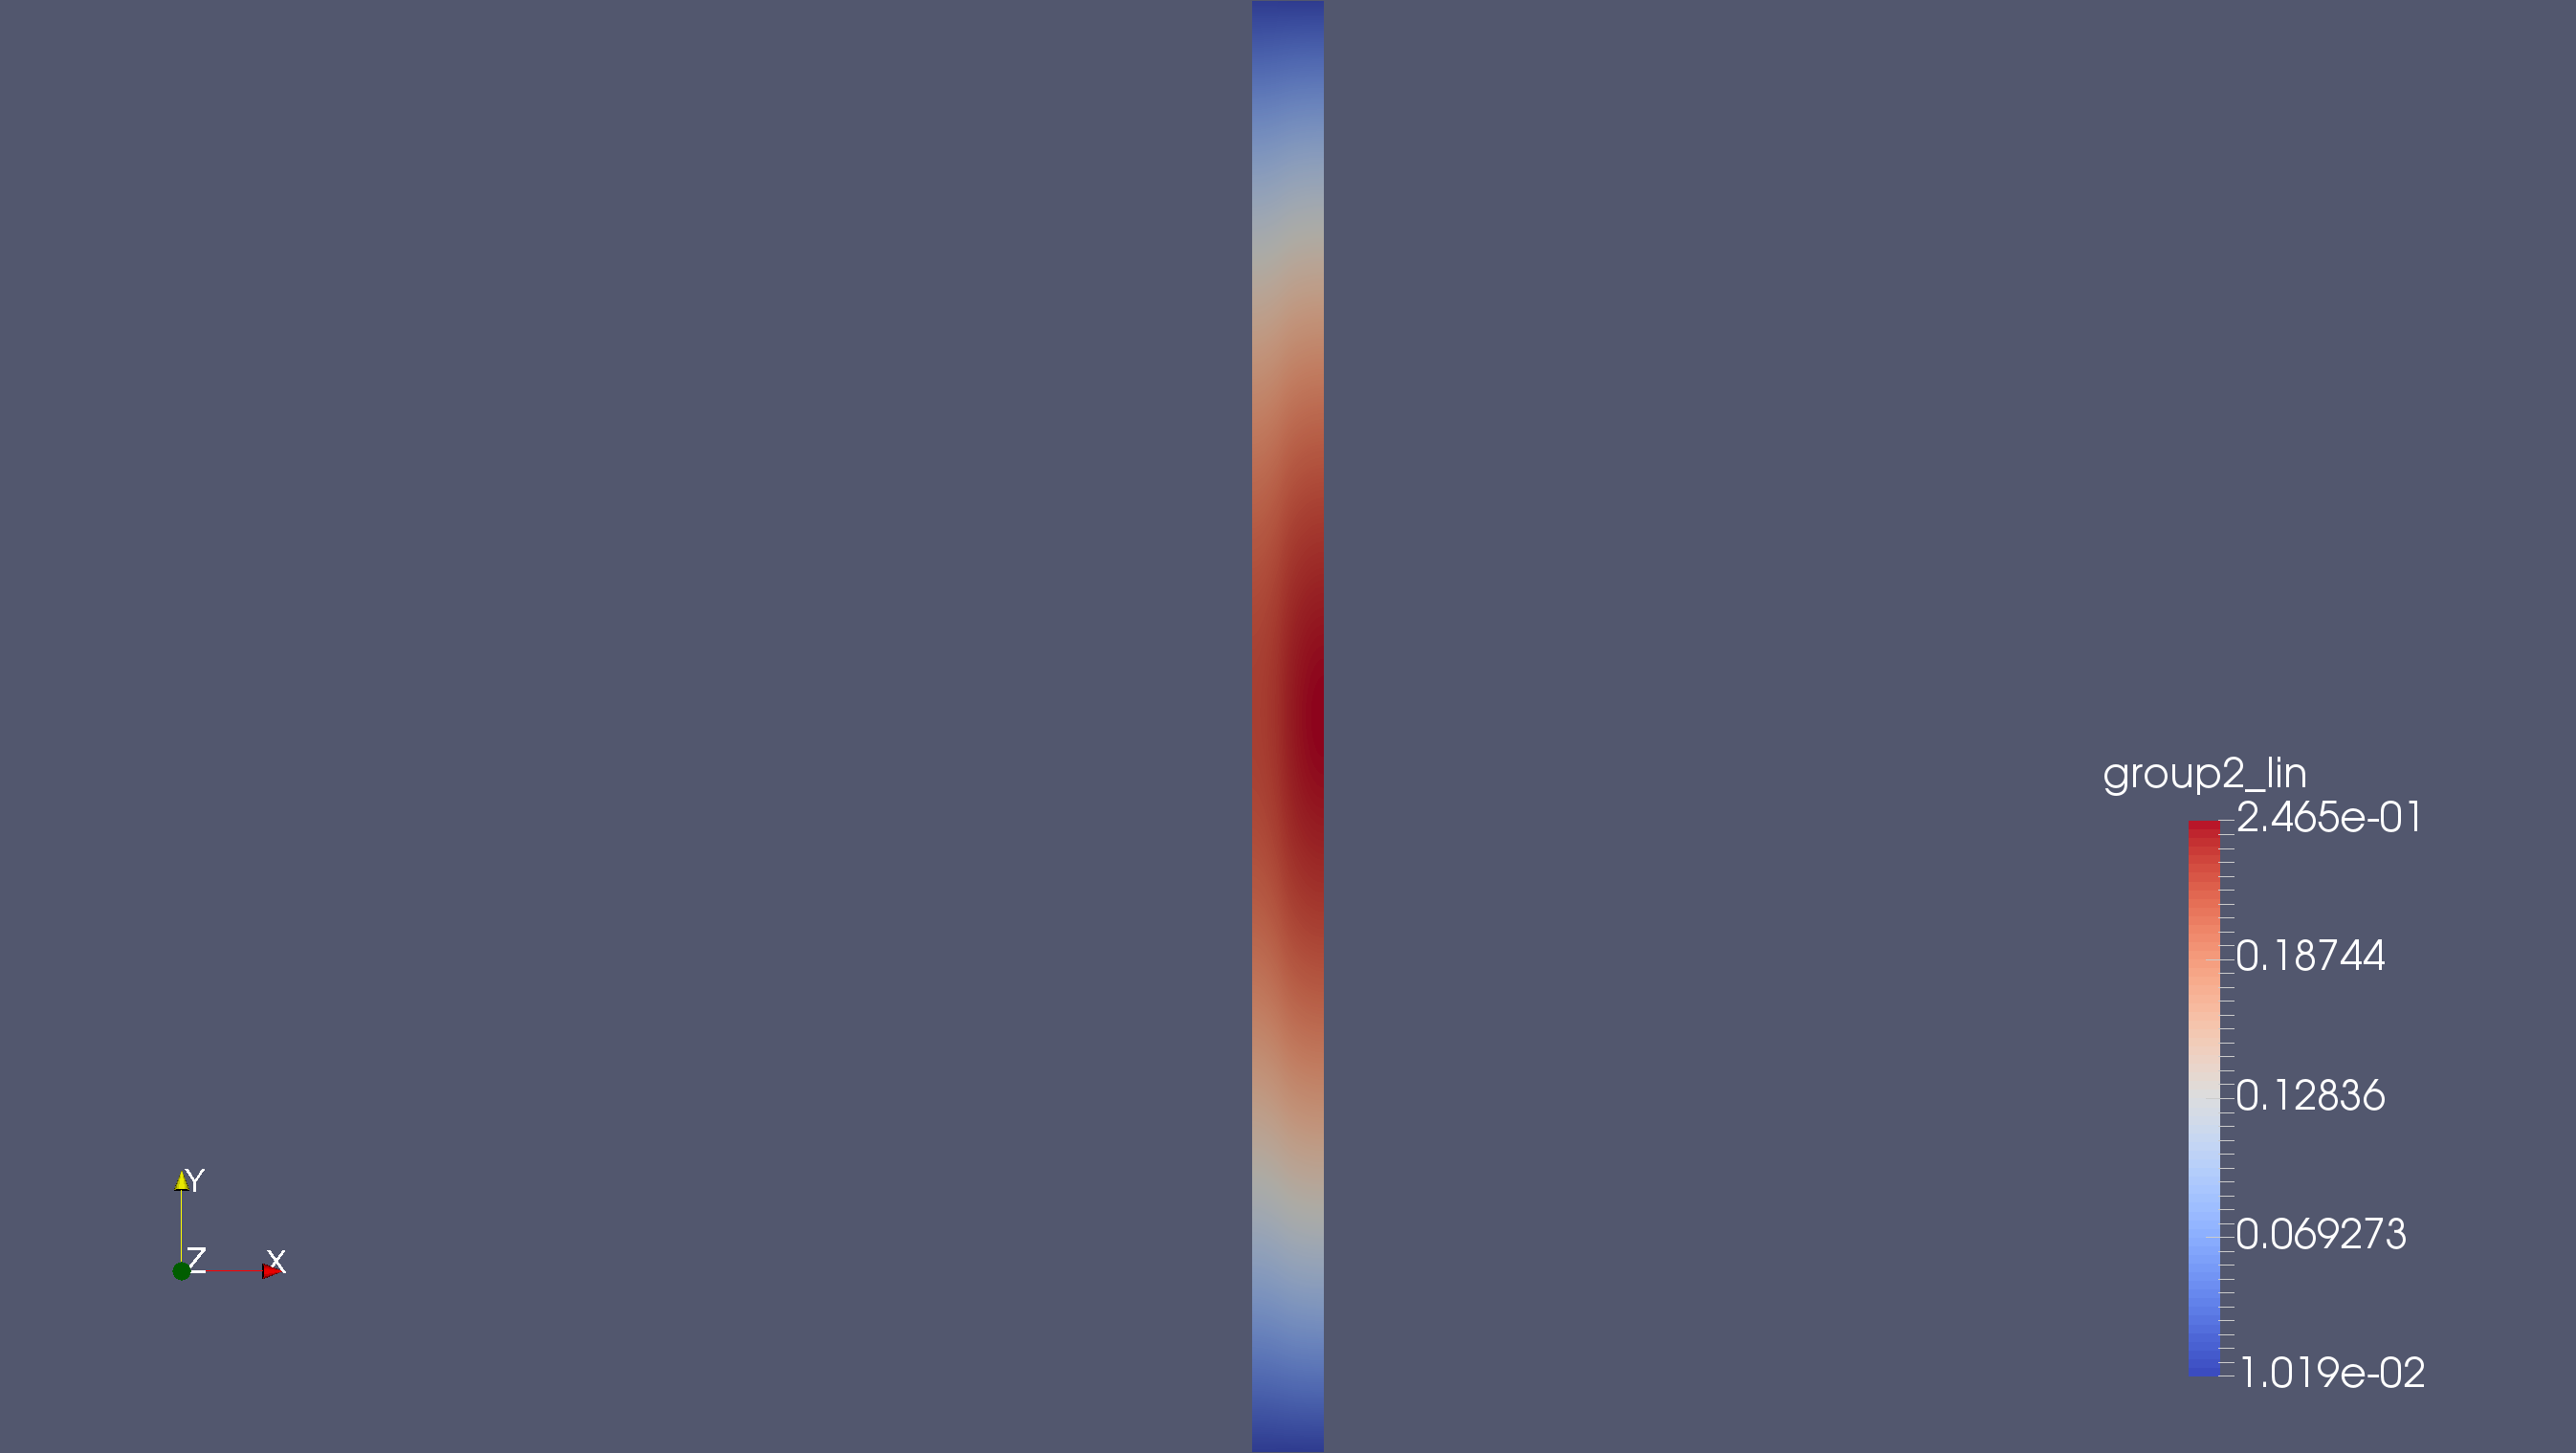
\includegraphics[width=.5\textwidth]{dg_group2.png}
  \caption{Thermal group neutron flux for Discontinuous Galerkin discretization}
  \label{fig:dg_group2}
\end{figure}

\FloatBarrier

\subsection{DG Temperature with Moderator Heat Source}

The \gls{MSR} model can be modified by adding a heat source in the moderator
corresponding to gamma heating and neutron irradiation \cite{robertson_conceptual_1971}.

Introduction of the moderator heat source further modifies the reactor
temperature profile as shown in
\cref{fig:dg_mod_source_temperature,fig:dg_mod_source_temperature_outlet}. Without
the moderator heat source, the maximum temperature in the reactor for \gls{CG}
and \gls{DG} discretizations is 992 and 1119 K respectively. These maxima both
occur at the reactor outlet and are more or less uniform over the radial
coordinate. However, with the addition of the moderator heat source, the reactor
temperature maximum rises to a somewhat absurd 1615 K (this is only 88 K below
the boiling point of \gls{FLiBe}). The location of the maximum is in the top right
corner of the simulation domain, corresponding to the middle of the graphite
moderator in a periodic lattice arrangement.

%% \begin{figure}[H]
\begin{figure}[htpb]
  \centering
  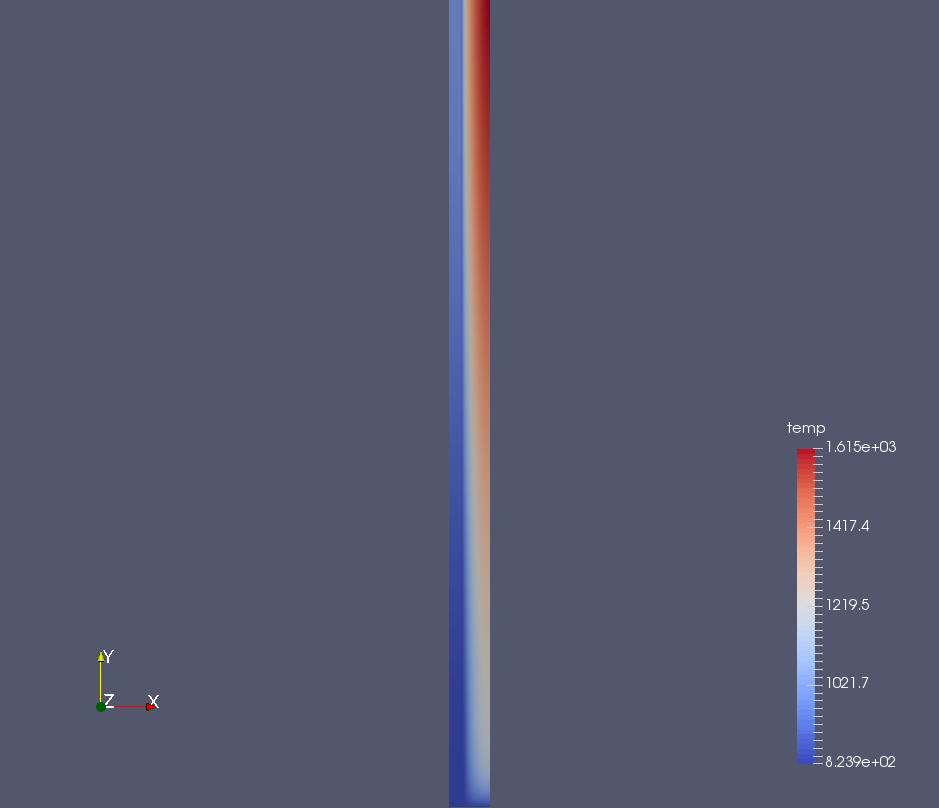
\includegraphics[width=.5\textwidth]{dg_mod_source_temperature_full_domain.png}
  \caption{Temperature for Discontinuous Galerkin discretization with moderator
    heat source}
  \label{fig:dg_mod_source_temperature}
\end{figure}

The temperature profile at the top of the reactor is no longer uniform with
respect to the radial coordinate as shown in
\cref{fig:dg_mod_source_temperature_outlet}. From the right edge of the
simulation domain (r = R$_2$), the graphite temperature decreases from its
maximum value of 1615 K to a value of about 1200 K at the fuel/graphite
interface. At the interface, perhaps due to the \gls{DG} discretization and the
order of magnitude difference in diffusion coefficients, there is a shock and
temperature oscillations in the fuel. After the oscillations are damped, the
fuel outlet temperature is uniform between r = 0 and 1.2 cm at a value of
approximately 990 K. This corresponds fairly closely to the outlet temperature
calculated in the isotropically stabilized \gls{CG} simulation, but the
correspondence is believed to be purely coincidental.

%% \begin{figure}[H]
\begin{figure}[htpb]
  \centering
  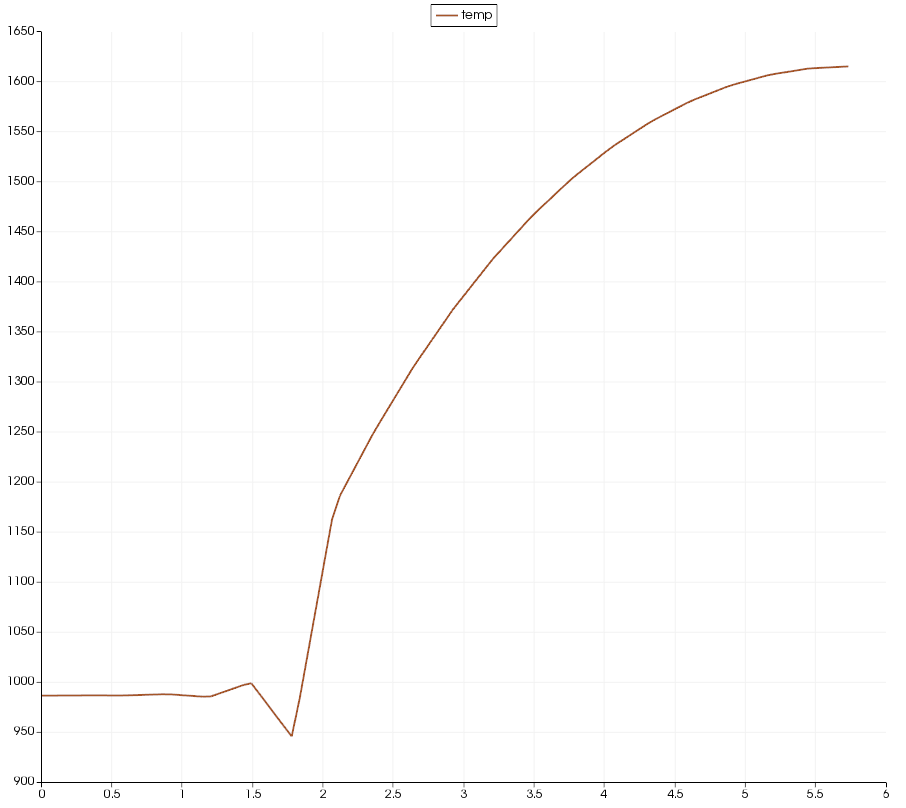
\includegraphics[width=.5\textwidth]{dg_mod_source_temperature_outlet.png}
  \caption{Fuel outlet temperature profile for Discontinuous Galerkin
    discretization with moderator heat source}
  \label{fig:dg_mod_source_temperature_outlet}
\end{figure}

\Cref{fig:dg_mod_source_group1,fig:dg_mod_source_group2} show the neutron fluxes
for the moderator heat source simulation case. Spatial shapes are the same as
the previous two simulation cases; howevever, the flux magnitudes are
less. A comparison of maximum flux magnitudes between the three simulation cases
is shown in \cref{tab:max_fluxes}.

%% \begin{figure}[H]
\begin{figure}[htpb]
  \centering
  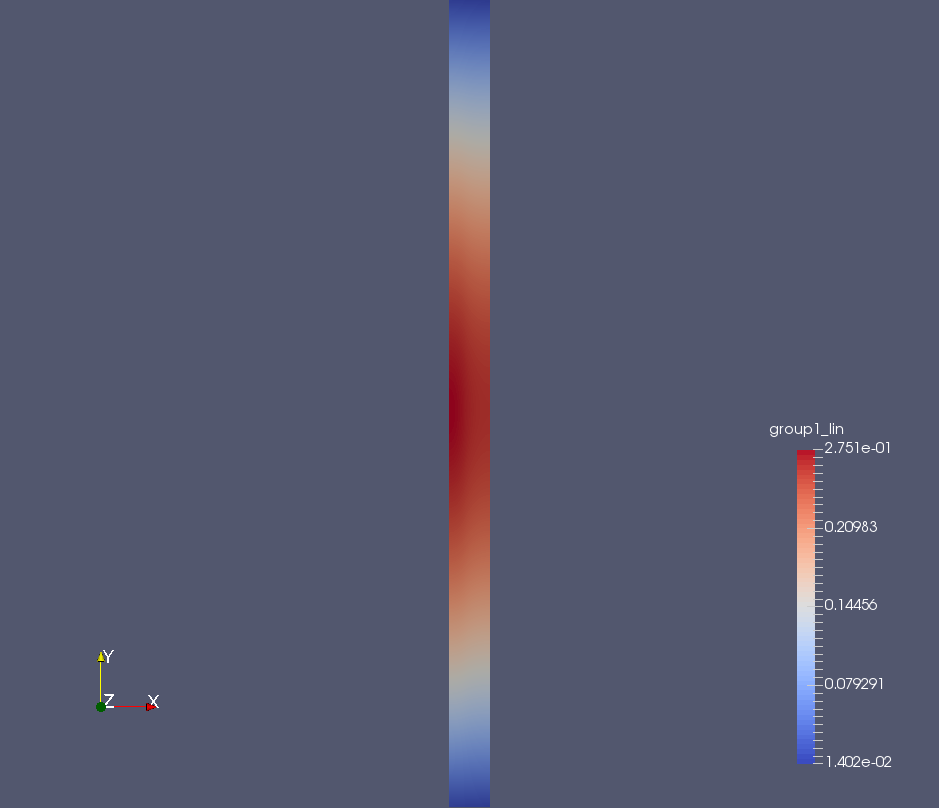
\includegraphics[width=.5\textwidth]{dg_mod_source_group1.png}
  \caption{Fast group neutron flux for Discontinuous Galerkin discretization
    with moderator heat source}
  \label{fig:dg_mod_source_group1}
\end{figure}

%% \begin{figure}[H]
\begin{figure}[htpb]
  \centering
  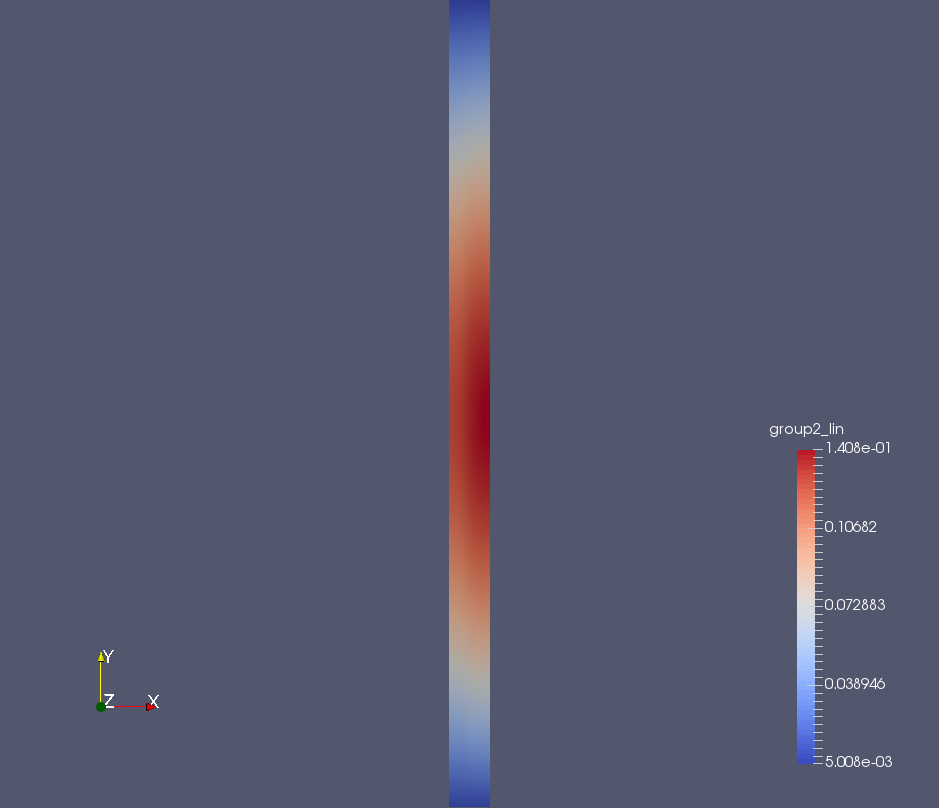
\includegraphics[width=.5\textwidth]{dg_mod_source_group2.png}
  \caption{Thermal group neutron flux for Discontinuous Galerkin discretization
    with moderator heat source}
  \label{fig:dg_mod_source_group2}
\end{figure}

\begin{table}[htpb]
    \begin{center}
      \begin{tabular}{l|c|c}
        Simulation Case & Maximum Fast Flux ($10^{15}\frac{\#}{cm^2s}$) & Maximum Thermal
        Flux ($10^{15}\frac{\#}{cm^2s}$)\\
        \hline \hline
        \gls{CG} & 3.488 & 1.785 \\
        \gls{DG} & 4.700 & 2.465 \\
        \gls{DG} with moderator source & 2.751 & 1.408 \\
      \end{tabular}
    \end{center}
    \caption{Maximum fluxes for different simulation cases}
    \label{tab:max_fluxes}
\end{table}

\FloatBarrier
\clearpage
\printglossary[type=\acronymtype]
\bibliographystyle{unsrt}
\bibliography{Moltres}
\end{document}
